\section{Mobile Application}

Another one of our tasks was to create a mobile application that fetches data from the respective
device and sends data to a \textit{Kafka} topic which subsequently invokes a \textit{serverless
function} to finally persist that data in a \textit{MongoDB} database. To approach this topic we
first did some research on current possibilities on creating cross platform mobile applications and
the general feasibility of the task at hand. It became quite apparent early on that the desired
design for the application is not possible on \textit{iOS}.

The idea for the design of the app is actually rather simple. Get data from the device, no matter if
the application is in the foreground, background or the screen is off and the device subsequently
in standby mode. On \textit{Android} this can be realised easily with a so called
\textit{ForegroundService}. On \textit{iOS} going for the same approach is difficult because of its
restrictions on background tasks. While obviously applications like music players can run in the
background on that platform, achieving the same for a highly battery intensive app like the one we
are developing, is more or less impossible.

Mainly for that reason we actually chose to go for a cross platform mobile application, so we can
have a fully supported \textit{Android} version and also an \textit{iOS} version with limited
functionality.

The versions of the mobile application for the two major phone operating systems not only differ
architecturally, they also have access to different sensors. On \textit{Android} we support the
following set of sensors: CPU frequency, proximity, acceleration, rotation, pressure, orientation,
gravity, illuminance, rate of rotation, rate of rotation uncalibrated, magnetic field and magnetic
field uncalibrated. While on \textit{iOS} the following sensors are supported: acceleration,
orientation, rotation rate, gravity, pressure and magnetic field.

Finding the ideal tool for our job of creating an application supporting both \textit{iOS} and
\textit{Android} seemed at first pretty easy. We chose to use \textit{React Native}
\cite{react-native} as we both already had experience with \textit{React} \cite{react} itself and
the approach to UI design in \textit{React Native} seemed equally elegant.

Getting started with \textit{React Native} was rather fast and effortless, the same however could
not be said anymore once we progressed further with the project. At first things were looking good
as the UI did properly respond to data from sensors but as we added more and more data for
display, the UI got more and more sluggish, to the point that it could not be considered usable
anymore. Unfortunately this was not the only problem.

By nature the application relies heavily on native code. The main culprit for this is the
\textit{ForegroundService} on \textit{Android}. \textit{React Native} has a so called
\textit{bridge} for communication between native code and the UI. Our application
uses that bridge heavily for retrieving information from the service and also to push data to the
service.

Once we fully implemented the settings view and were basically finished with the application, the
app started to crash constantly on \textit{Android}. Unfortunately the tooling of \textit{React
Native} really does not help with debugging fatal crashes. So we had to make a conscious decision
whether we want to continue with \textit{React Native} or start over with something else entirely.

In the end we concluded to search for other frameworks as we deemed \textit{React Native} as
incompatible for our task. We then decided on using \textit{Flutter}. \textit{Flutter} is a modern
cross platform mobile application framework by \textit{Google}. \textit{Flutter} compiles down to
native code and therefore should have a performance advantage compared to \textit{React Native}.

As with any new programming language, \textit{Dart} - the language behind \textit{Flutter} - took
some time to get used to and be productive with. After a while however, the process of designing user
interfaces with \textit{Flutter} and writing logic was rather seamless. Fortunately the native part
of the \textit{React Native} application could almost fully be reused for the \textit{Flutter}
version of the app. The surprisingly easy to use \textit{bridge} between native code and
\textit{Dart} in \textit{Flutter} made the transition from \textit{React Native} regarding native
code on \textit{Android} hassle free.

One of the reasons we first chose to use \textit{React Native} was the extensive community support.
Getting sensor data from almost all supported sensors on \textit{iOS} was as simple as including a
package. The same cannot be said about \textit{Flutter}. For that reason we also had to write some
native code for \textit{iOS}, which splits the code base even further.

The finished application now contains five Views:

\begin{figure}[H]
  \centering
  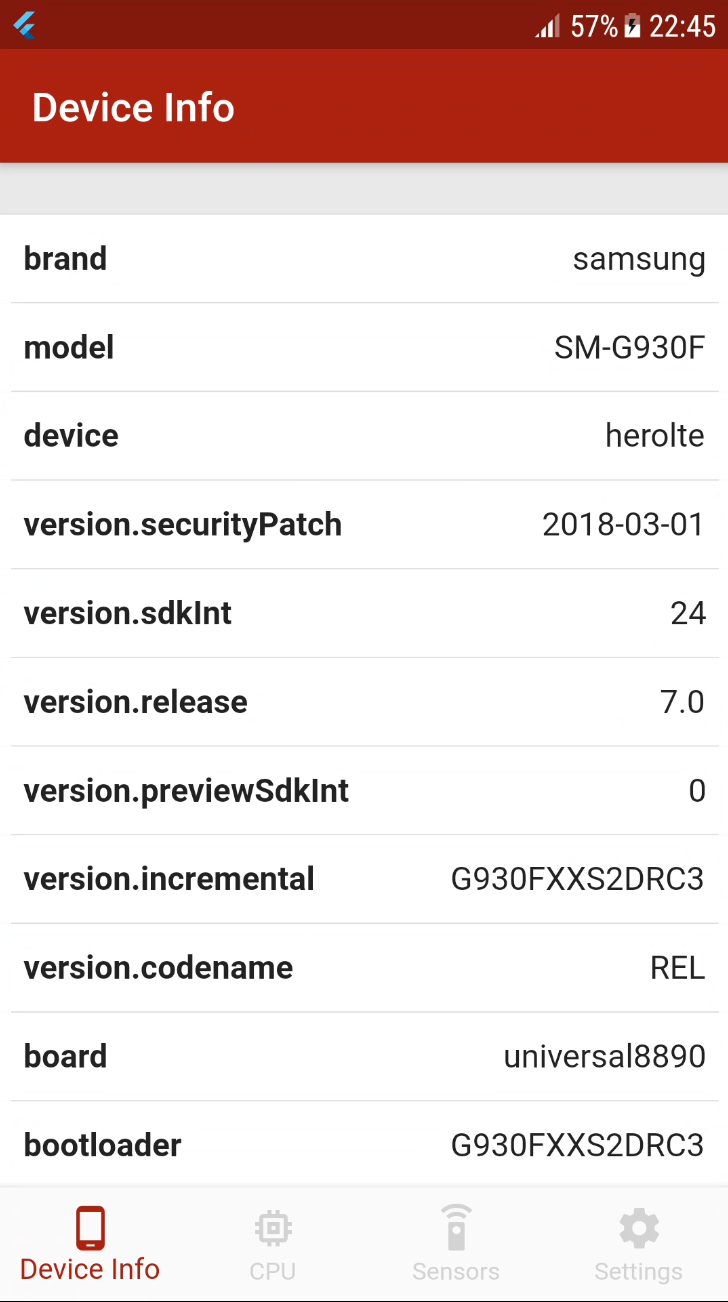
\includegraphics[height=20em]{mobile-device-info}
  \caption{\texttt{Device Info} contains various information about the running system.}
\end{figure}

\begin{figure}[H]
  \centering
  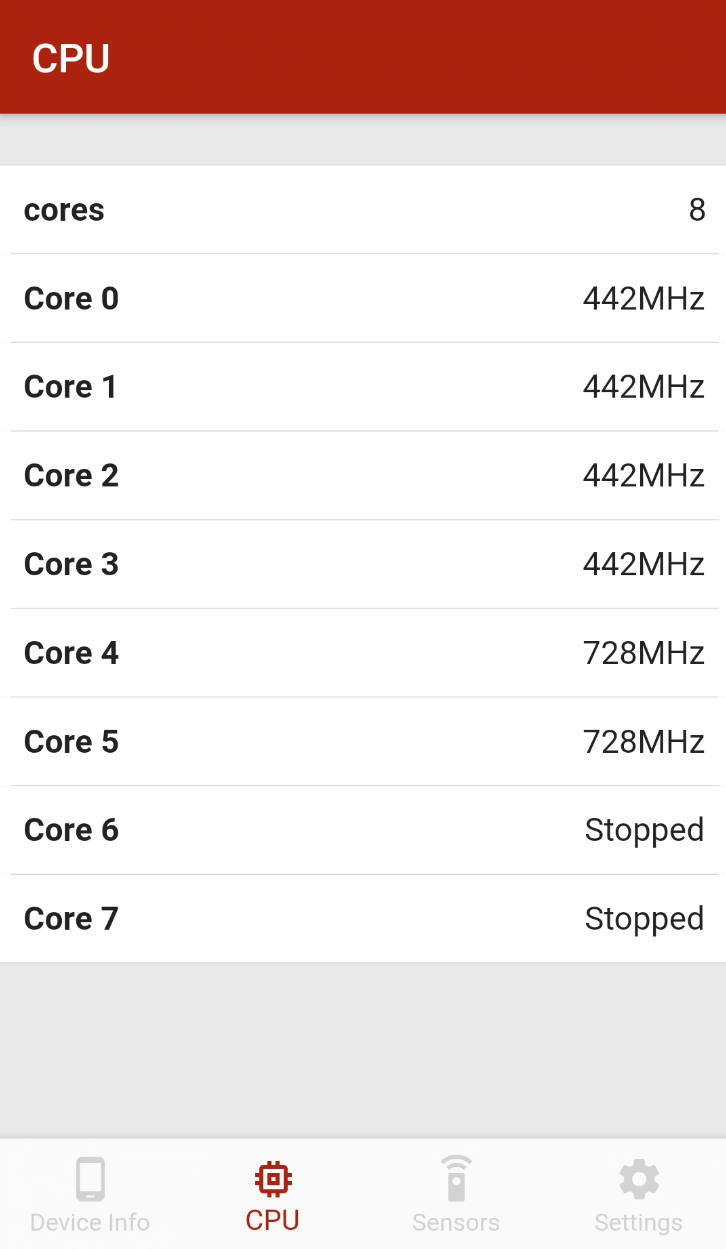
\includegraphics[height=20em]{mobile-cpu}
  \caption{CPU shows the amount of cores available and the frequency they are currently
  running at, if they are running at all. This view, however, is only available on \textit{Android}
  due to limitations on retrieval of CPU information on \textit{iOS}.}
\end{figure}

\begin{figure}[H]
  \centering
  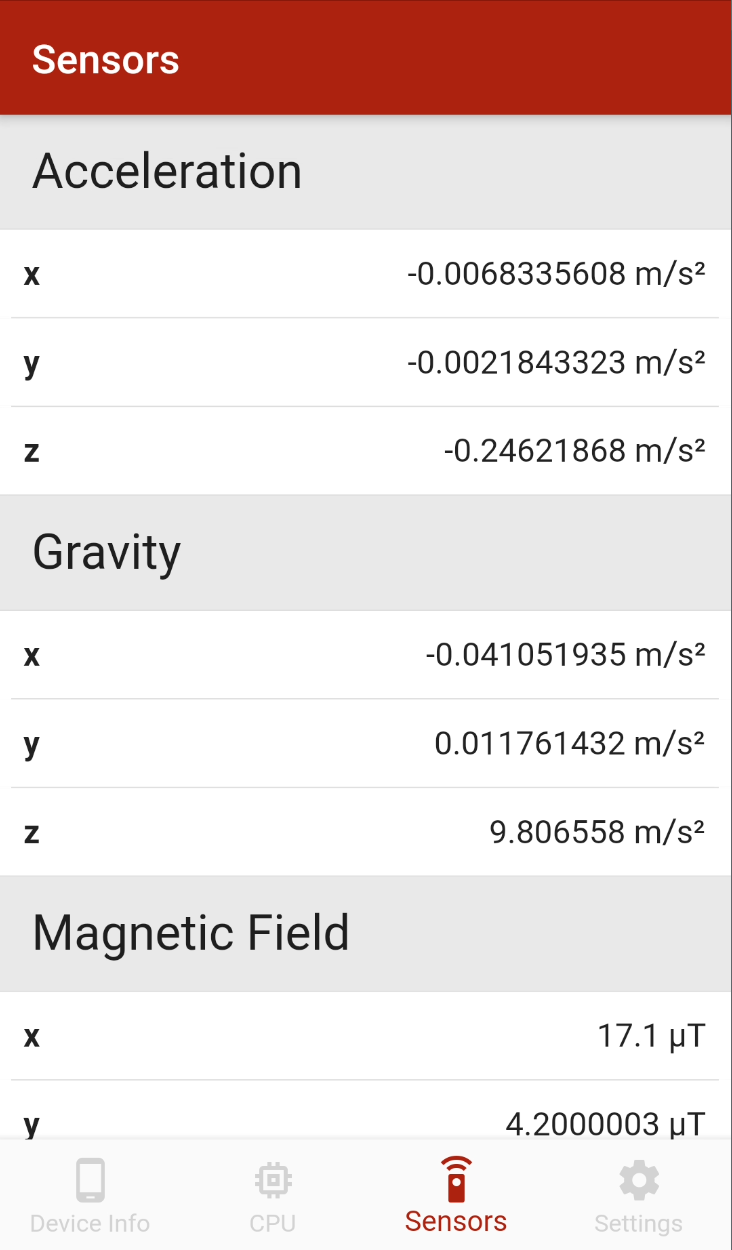
\includegraphics[height=20em]{mobile-sensors}
  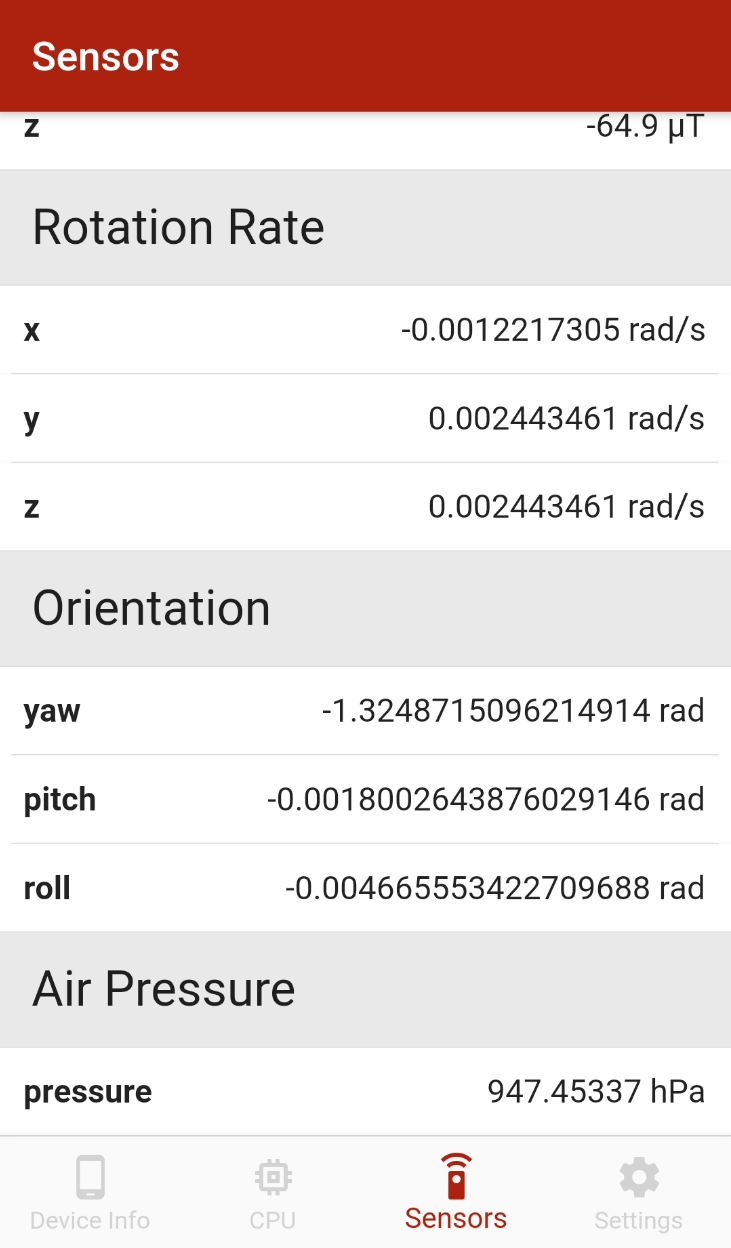
\includegraphics[height=20em]{mobile-sensors-2}
  \caption{\texttt{Sensors} lists various sensors on both platforms.}
\end{figure}

\begin{figure}[H]
  \centering
  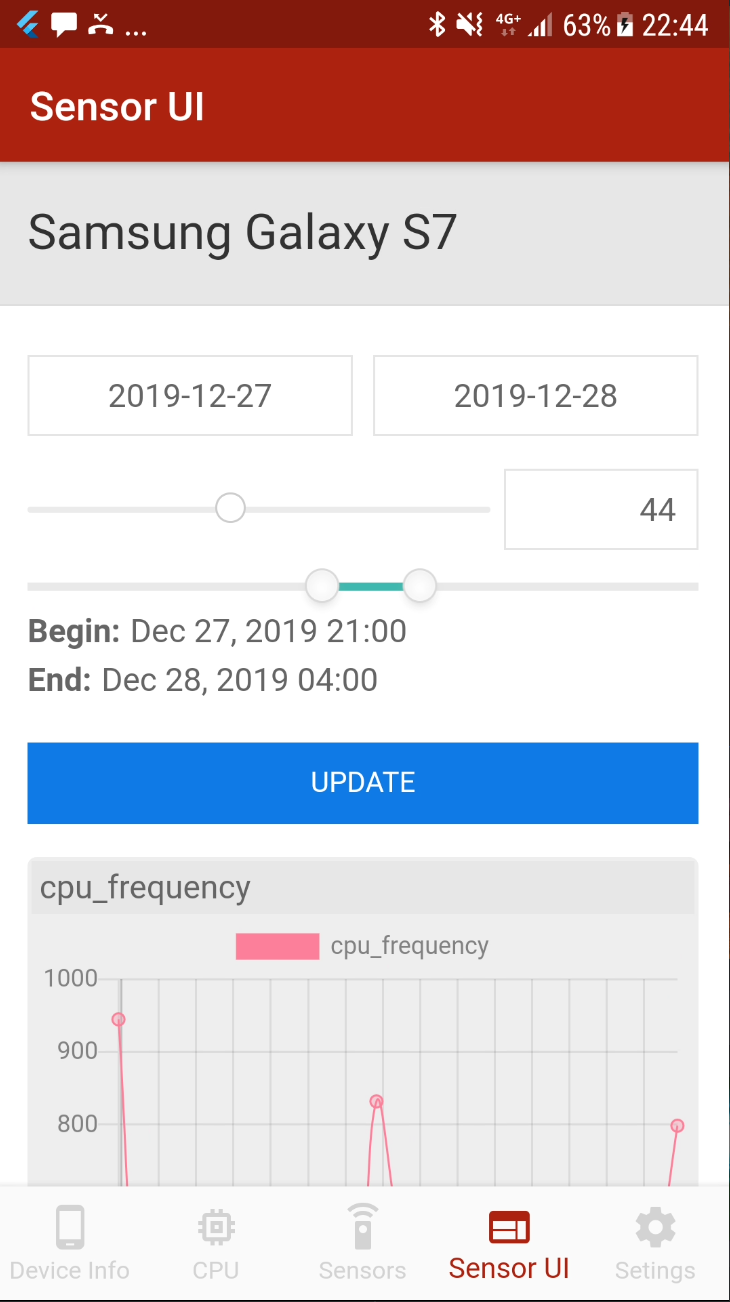
\includegraphics[height=20em]{mobile-ui}
  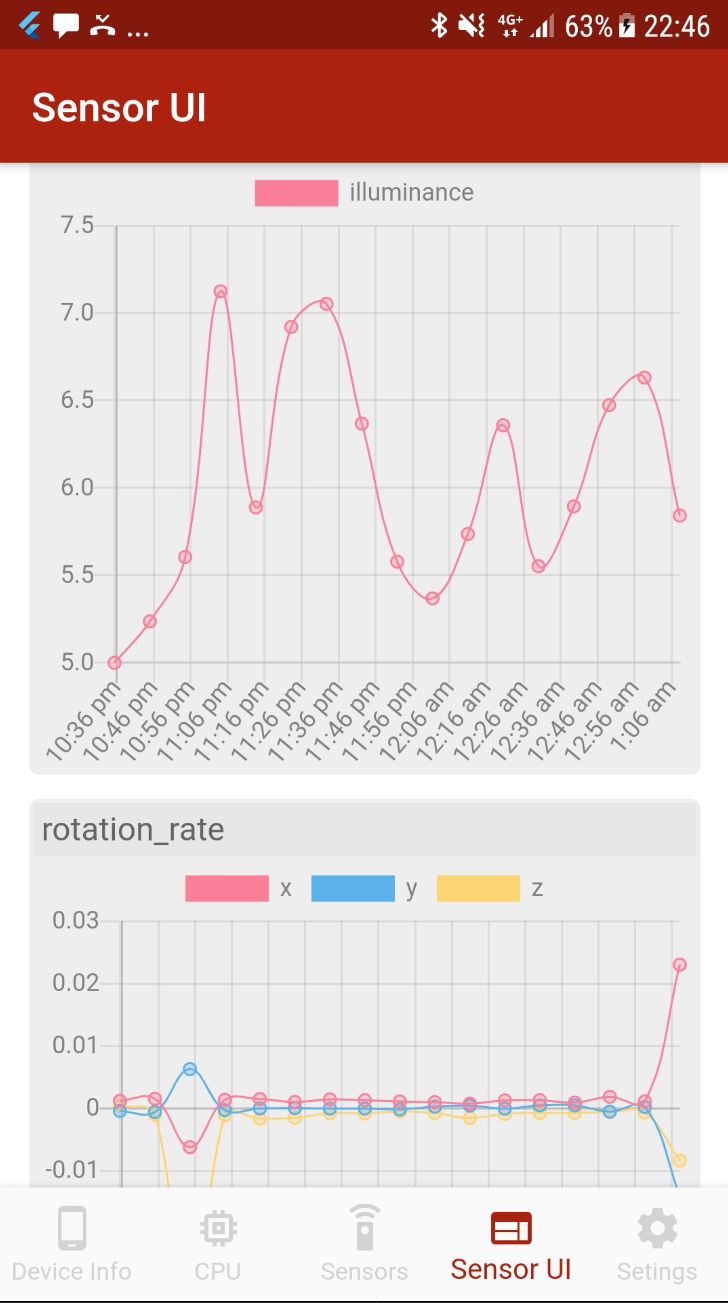
\includegraphics[height=20em]{mobile-ui-sensors}
  \caption{\texttt{Sensor UI} shows the UI (explained in \autoref{sec:ui}) embedded in the application.}
\end{figure}

\begin{figure}[H]
  \centering
  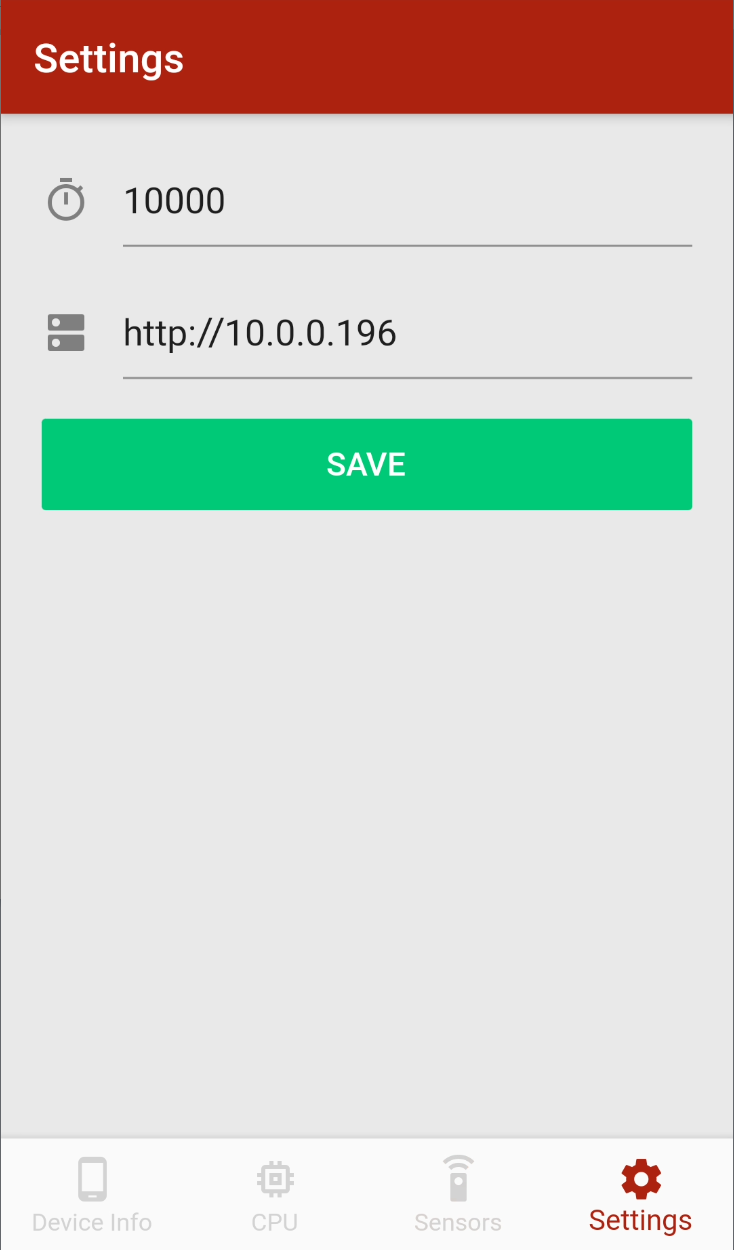
\includegraphics[height=20em]{mobile-settings}
  \caption{\texttt{Settings} gives the user the ability to modify the interval of sending data to the
  server and the URL where the server is located.}
\end{figure}

The most important part about the application however is sending data to a \textit{Kafka} topic.
\textit{Kafka} then invokes a serverless function. The task of the serverless function is then to
push the data into our \textit{MongoDB} database. To achieve this we wrap all data into categories
and send them to the specific topic in \textit{Kafka} via \textit{JSON}.
